\documentclass[12pt]{beamer}
\usetheme{Dresden}
\usepackage[utf8]{inputenc}
\usepackage[spanish]{babel}
\usepackage{amsmath}
\usepackage{amsfonts}
\usepackage{amssymb}
\usepackage{graphicx}
\usepackage{caption}
\author{Diego R. Zagals}
\title{DataStax on WeatherStation}
\setbeamercovered{transparent} 
\setbeamertemplate{navigation symbols}{} 
\logo{
\includegraphics[scale=0.075]{almalog_300dpi.jpg} } 
\institute{El Atacama Large Millimeter/submillimeter Array } 
\date{\today} 
\subject{OracleDB Migration to Cassandra} 

\begin{document}

\begin{frame}
\titlepage
\begin{figure}[Antennas]
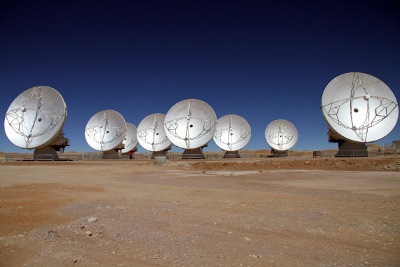
\includegraphics[scale=0.5]{antennas.jpg} 
\label{Antennas}
\end{figure}
\end{frame}

%\begin{frame}
%\tableofcontents
%\end{frame}

\begin{frame}
\begin{block}{Index}
\begin{itemize}
\item WeatherStation
\item Today
\item Objectives
\item At this point
\end{itemize}
\end{block}
\end{frame}

\begin{frame}
\begin{block}{WeatherStation}
\begin{itemize}
\item The weather station data is not only used to correct antenna pointing during scientific observations
\item But also used by other applications in ALMA and other institutions distributed in the world. 
\item The amount of concurrent requests could degrade the performance of the web services and increase the latency of data delivery
\end{itemize}
\end{block}
\end{frame}

\begin{frame}
\begin{columns}
\column{.5\textwidth}
\begin{figure}
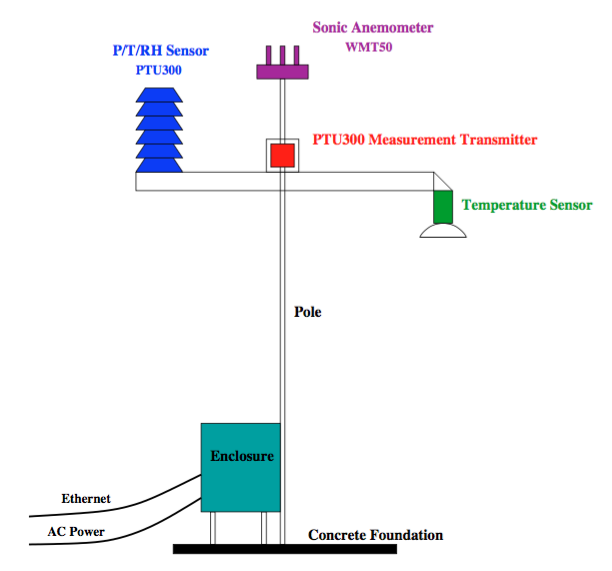
\includegraphics[scale=0.3]{Diagrama.png}\vspace*{10pt}
\captionsize\tiny Figure 1: Sketch of a standard weather instrument installation.
\label{Diagram}
\end{figure}
\column{.5\textwidth}
\begin{figure}
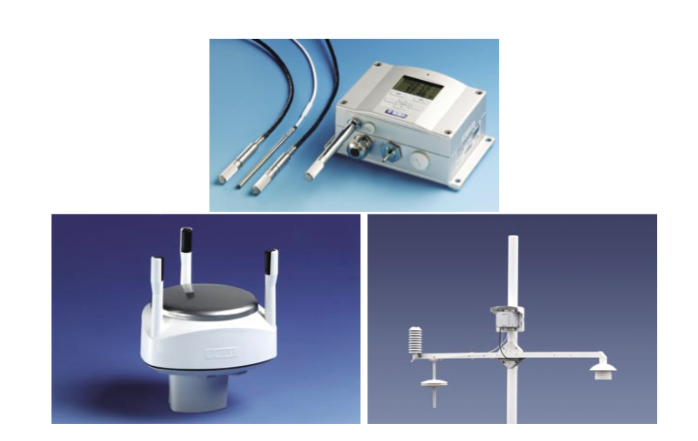
\includegraphics[scale=0.2]{Sensores.png}\vspace*{10pt}
\captionsize\tiny Figure 2: Clockwise from top: PTU300 P, T, and RH sensor, HMT330MIK meteorological installation kit, and WMT50 sonic anemometer.
\label{Sensor}
\end{figure}
\end{columns}
\end{frame}

\begin{frame}{Today}
\begin{itemize}
\item ~6 years ago, 3 weather stations
\item 11 weather stations -$>$ too many data insertions into the Oracle relational database
\item Migrate the persistent storage of weather data into Cassandra cluster
\end{itemize}
\end{frame}

\begin{frame}
\begin{columns}
\column{.2\textwidth}
\begin{center}
\begin{figure}[Schematic]
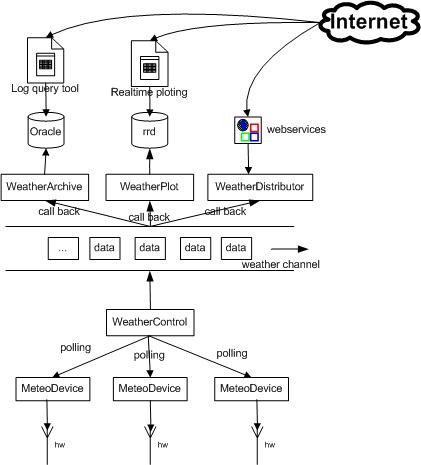
\includegraphics[scale=0.4]{WeatherStation_esquemas.jpg} \vspace*{10pt}
\captionsize\tiny Figure 3: System Schematic.
\label{System Schematic}
\end{figure}
\end{center}
\column{.5\textwidth}
\begin{center}
\begin{figure}[DB]
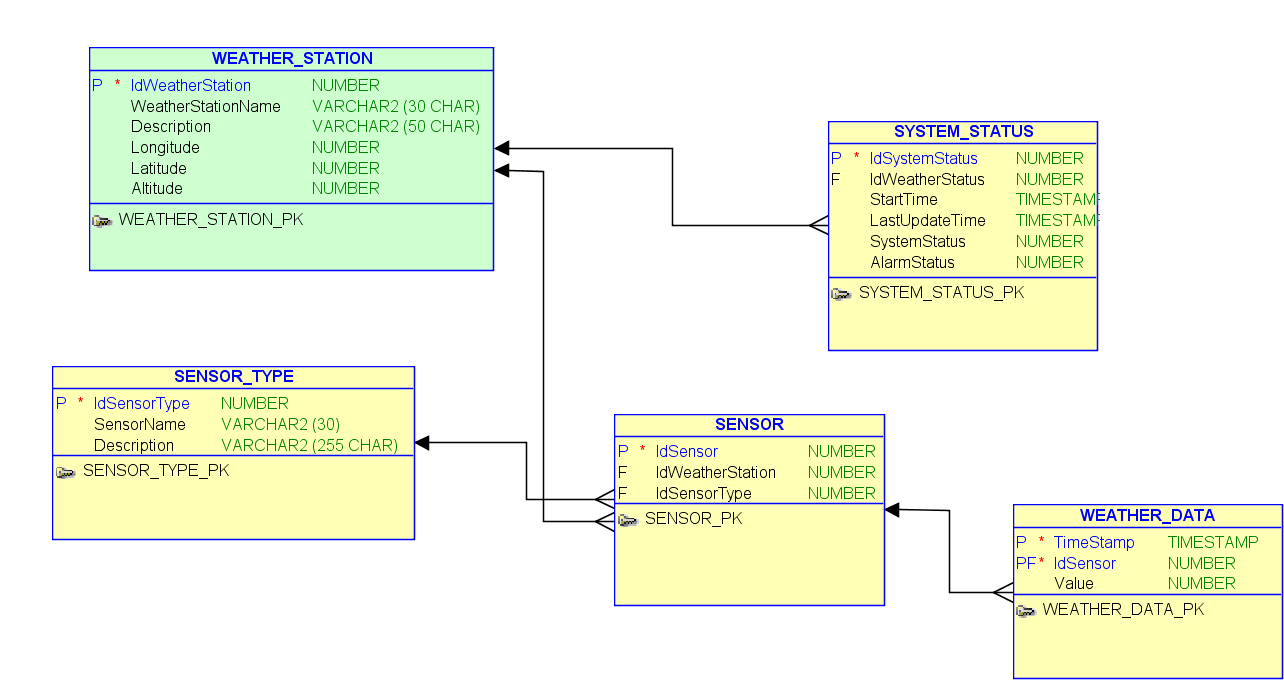
\includegraphics[scale=0.15]{WeatherStation.png} \vspace*{10pt}
\captionsize\tiny Figure 4: Relational DB.
\label{DB}
\end{figure}
\end{center}
\end{columns}
\end{frame}

\begin{frame}{Objectives}
\begin{block}{Improvements to the standalone weather station platform.}
\begin{itemize}
\item Migrate weather data storage from Oracle to Cassandra
\item Improve the usability of the existent web interface
\item Improve the performance of the web service.
\end{itemize}
\end{block}
\begin{columns}
\column{.1\textwidth}

\includegraphics[scale=0.05]{Cassandra_logo.png} \label{Cassandra}
\column{.5\textwidth}

\includegraphics[scale=0.4]{DataStax_Logo.png} \label{DataStax}
\end{columns}
\end{frame}

\begin{frame}{At this point}
\large RecentWork: 
\vspace*{-15pt}
\begin{center}
%\begin{figure}[Tables]
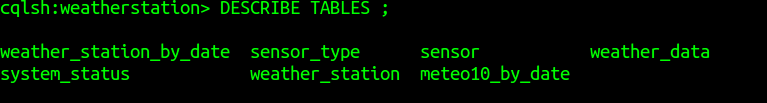
\includegraphics[scale=0.4]{tables.png} \vspace*{10pt}
%\captionsize\tiny Figure 5: Tables on WeatherStation KEYSPACE.
%\label{Tables}
%\end{figure}
%\begin{figure}[Meteo10]
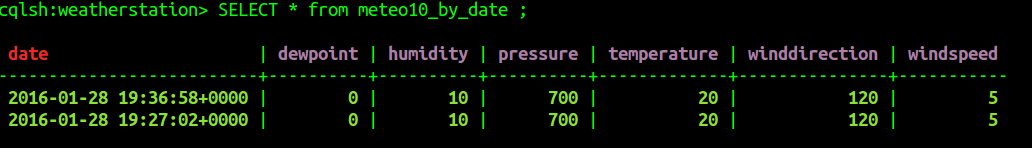
\includegraphics[scale=0.3]{meteo10_by_date.png} \vspace*{10pt}
%\captionsize\tiny Figure 6: INSERT data on table meteo10_by_date.
%\label{Meteo10}
%\end{figure}
\end{center}
\normalsize ...FeedBack :)
\end{frame}

\end{document}
